%
% 6.006 problem set 8 solutions template
%

\documentclass[12pt,twoside]{article}

% 添加中文支持
\usepackage[fontset=windows]{ctex}
\usepackage{fontspec}
\usepackage{amsmath}  % 确保amsmath包被引入
\usepackage{mathtools} % 添加对dcases环境的支持
\setmainfont{Times New Roman}
% 如果您使用的是 Windows 系统,并且安装了思源宋体或其他中文字体,可以尝试以下设置
% \setCJKmainfont{Source Han Serif CN}
% \setCJKsansfont{Source Han Sans CN}
% \setCJKmonofont{Source Han Sans CN}

% 该模板是《算法设计与分析》课程习题,修改自MIT 6.006
%2021.1.27 增加了中文
\newcommand{\name}{}

\usepackage{amssymb}
\usepackage{amsmath}
\usepackage{graphicx}
\usepackage{latexsym}
\usepackage{times,url}
\usepackage{cprotect}
\usepackage{listings}
\usepackage{graphicx}
\usepackage[table]{xcolor}
\usepackage[letterpaper]{geometry}
\usepackage{enumerate}
\usepackage{forest}
\usepackage{tikz-qtree}
\usepackage{tikz}       % 用于画图的包
\usepackage[linesnumbered,lined,commentsnumbered,ruled]{algorithm2e}  % 用于写伪代码
\usepackage{xeCJK} 			% 写中文要用到
\newcommand{\forcond}{$i=0$ \KwTo $n$} %用于伪代码
\SetKwProg{Fn}{Function}{}{end}
\SetAlgoLongEnd

%===========================段落设置================================================ 
\usepackage{setspace} 
\setlength{\parindent}{2em} 
\setlength{\parskip}{1ex plus 0.5ex minus 0.2ex} 
\linespread{1.35}

\renewcommand\figurename{图} %
\renewcommand\tablename{表}%
%%%%%

\newcommand{\profs}{{\bf 教师}: 杜嘉欣}
\newcommand{\subj}{6.006}
\newcommand{\ttt}[1]{{\tt\small #1}}

\definecolor{dkgreen}{rgb}{0,0.6,0}
\definecolor{dkblue}{rgb}{.2,.2,1}
\definecolor{gray}{rgb}{0.5,0.5,0.5}
\definecolor{mauve}{rgb}{0.58,0,0.82}

\lstset{
  language=Python,
  aboveskip=1pc,
  belowskip=1pc,
  basicstyle={\footnotesize\ttfamily},
  numbers=left,
  showstringspaces=false,
  numberstyle={\tiny\color{gray}\ttfamily},
  keywordstyle={\color{dkblue}\ttfamily},
  commentstyle={\color{dkgreen}\ttfamily},
  stringstyle={\color{mauve}\ttfamily},
}

% \lstset{
%   language=Python,
%   aboveskip=1pc,
%   belowskip=1pc,
%   basicstyle={\bf\color{white}\ttfamily},
%   numbers=left,
%   showstringspaces=false,
%   numberstyle={\bf\small\color{lightgray}\ttfamily},
%   keywordstyle={\bf\color{cyan}\ttfamily},
%   commentstyle={\bf\color{green}\ttfamily},
%   stringstyle={\bf\color{mauve}\ttfamily},
% }


\tikzset{
  % every node/.style={minimum width=2em,draw,circle},
  % level 1/.style={sibling distance=2cm},
  level distance=1cm,
  edge from parent/.style=
  {draw,edge from parent path={(\tikzparentnode) -- (\tikzchildnode)}},
}
\usetikzlibrary{shapes}

\newif\ifHideSolutions
\newcommand{\solution}[1]{\color{dkgreen}\textbf{解答: }#1\color{black}}
\newcommand{\commonmistakes}[1]{{\color{dkblue}\textbf{常见错误: }#1}}
\newcommand{\rubric}[1]{\color{dkgreen}{\bf 说明:} #1\color{black}}

% \HideSolutionsfalse
% \ifHideSolutions
%   \renewcommand{\solution}[1]{}
%   \renewcommand{\rubric}[1]{}
% \fi

\newlength{\toppush}
\setlength{\toppush}{2\headheight}
\addtolength{\toppush}{\headsep}

\newcommand{\htitle}[2]{\noindent\vspace*{-\toppush}\newline\parbox{\textwidth}
{\textit{算法分析与设计}\hfill\name\newline
{\bf 浙江工业大学} \hfill #2\newline
\profs\hfill #1 \\[-3.5ex]\newline
\mbox{}\hrulefill\mbox{}}\vspace*{1ex}\mbox{}\newline
\begin{center}{\Large\bf #1}\end{center}}

\newcommand{\handout}[2]{\thispagestyle{empty}
 \markboth{#1}{#1}
 \pagestyle{myheadings}\htitle{#1}{#2}}

\newcommand{\lecture}[3]{\thispagestyle{empty}
 \markboth{Lecture #1: #2}{Lecture #1: #2}
 \pagestyle{myheadings}\htitle{Lecture #1: #2}{#3}}

\newcommand{\htitlewithouttitle}[2]{\noindent\vspace*{-\toppush}\newline\parbox{6.5in}
{\textit{算法分析与设计}\hfill#2\newline
浙江工业大学 \hfill 6.006\newline
\profs\hfill Handout #1\vspace*{-.5ex}\newline
\mbox{}\hrulefill\mbox{}}\vspace*{1ex}\mbox{}\newline}

\newcommand{\handoutwithouttitle}[2]{\thispagestyle{empty}
 \markboth{Handout \protect\ref{#1}}{Handout \protect\ref{#1}}
 \pagestyle{myheadings}\htitlewithouttitle{\protect\ref{#1}}{#2}}

\newcommand{\exam}[2]{% parameters: exam name, date
 \thispagestyle{empty}
 \markboth{\hspace{1cm}\subj\ #1\hspace{1in}Name\hrulefill\ \ }%
          {\subj\ #1\hspace{1in}Name\hrulefill\ \ }
 \pagestyle{myheadings}\examtitle{#1}{#2}
 \renewcommand{\theproblem}{Problem \arabic{problemnum}}
}
\newcommand{\examsolutions}[3]{% parameters: handout, exam name, date
 \thispagestyle{empty}
 \markboth{Handout \protect\ref{#1}: #2}{Handout \protect\ref{#1}: #2}
% \pagestyle{myheadings}\htitle{\protect\ref{#1}}{#2}{#3}
 \pagestyle{myheadings}\examsolutionstitle{\protect\ref{#1}} {#2}{#3}
 \renewcommand{\theproblem}{Problem \arabic{problemnum}}
}
\newcommand{\examsolutionstitle}[3]{\noindent\vspace*{-\toppush}\newline\parbox{6.5in}
{\textit{Introduction to Algorithms}\hfill#3\newline
Massachusetts Institute of Technology \hfill 6.006\newline
%Singapore-MIT Alliance \hfill SMA5503\newline
\profs\hfill Handout #1\vspace*{-.5ex}\newline
\mbox{}\hrulefill\mbox{}}\vspace*{1ex}\mbox{}\newline
\begin{center}{\Large\bf #2}\end{center}}

\newcommand{\takehomeexam}[2]{% parameters: exam name, date
 \thispagestyle{empty}
 \markboth{\subj\ #1\hfill}{\subj\ #1\hfill}
 \pagestyle{myheadings}\examtitle{#1}{#2}
 \renewcommand{\theproblem}{Problem \arabic{problemnum}}
}

\makeatletter
\newcommand{\exambooklet}[2]{% parameters: exam name, date
 \thispagestyle{empty}
 \markboth{\subj\ #1}{\subj\ #1}
 \pagestyle{myheadings}\examtitle{#1}{#2}
 \renewcommand{\theproblem}{Problem \arabic{problemnum}}
 \renewcommand{\problem}{\newpage
 \item \let\@currentlabel=\theproblem
 \markboth{\subj\ #1, \theproblem}{\subj\ #1, \theproblem}}
}
\makeatother


\newcommand{\examtitle}[2]{\noindent\vspace*{-\toppush}\newline\parbox{6.5in}
{\textit{算法分析与设计}\hfill#2\newline
浙江工业大学 \hfill  2024\newline
%Singapore-MIT Alliance \hfill SMA5503\newline
\profs\hfill #1\vspace*{-.5ex}\newline
\mbox{}\hrulefill\mbox{}}\vspace*{1ex}\mbox{}\newline
\begin{center}{\Large\bf #1}\end{center}}

\newcommand{\grader}[1]{\hspace{1cm}\textsf{\textbf{#1}}\hspace{1cm}}

\newcommand{\points}[1]{[#1 分]\ }
\newcommand{\parts}[1]
{
  \ifnum#1=1
  (1 part)
  \else
  (#1 parts)
  \fi
  \ 
}

\newcommand{\bparts}{\begin{problemparts}}
\newcommand{\eparts}{\end{problemparts}}
\newcommand{\ppart}{\problempart}

%\newcommand{\lg} {lg\ }

\setlength{\oddsidemargin}{0pt}
\setlength{\evensidemargin}{0pt}
\setlength{\textwidth}{6.5in}
\setlength{\topmargin}{0in}
\setlength{\textheight}{8.5in}


\newcommand{\Spawn}{{\bf spawn} }
\newcommand{\Sync}{{\bf sync}}

\renewcommand{\cases}[1]{\left\{ \begin{array}{ll}#1\end{array}\right.}
\newcommand{\cif}[1]{\mbox{if $#1$}}
\newcommand{\cwhen}[1]{\mbox{when $#1$}}

\newcounter{problemnum}
\newcommand{\theproblem}{题目 \theproblemsetnum-\arabic{problemnum}}
\newenvironment{problems}{
        \begin{list}{{\bf \theproblem. \hspace*{0.5em}}}
        {\setlength{\leftmargin}{0em}
         \setlength{\rightmargin}{0em}
         \setlength{\labelwidth}{0em}
         \setlength{\labelsep}{0em}
         \usecounter{problemnum}}}{\end{list}}
\makeatletter
\newcommand{\problem}[1][{}]{\item \let\@currentlabel=\theproblem \textbf{#1}}
\makeatother

\newcounter{problempartnum}[problemnum]
\newenvironment{problemparts}{
        \begin{list}{{\bf (\alph{problempartnum})}}
        {\setlength{\leftmargin}{2.5em}
         \setlength{\rightmargin}{2.5em}
         \setlength{\labelsep}{0.5em}}}{\end{list}}
\newcommand{\problempart}{\addtocounter{problempartnum}{1}\item}

\newenvironment{truefalseproblemparts}{
        \begin{list}{{\bf (\alph{problempartnum})\ \ \ T\ \ F\hfil}}
        {\setlength{\leftmargin}{4.5em}
         \setlength{\rightmargin}{2.5em}
         \setlength{\labelsep}{0.5em}
         \setlength{\labelwidth}{4.5em}}}{\end{list}}

\newcounter{exercisenum}
\newcommand{\theexercise}{Exercise \theproblemsetnum-\arabic{exercisenum}}
\newenvironment{exercises}{
        \begin{list}{{\bf \theexercise. \hspace*{0.5em}}}
        {\setlength{\leftmargin}{0em}
         \setlength{\rightmargin}{0em}
         \setlength{\labelwidth}{0em}
         \setlength{\labelsep}{0em}
        \usecounter{exercisenum}}}{\end{list}}
\makeatletter
\newcommand{\exercise}{\item \let\@currentlabel=\theexercise}
\makeatother

\newcounter{exercisepartnum}[exercisenum]
%\newcommand{\problem}[1]{\medskip\mbox{}\newline\noindent{\bf Problem #1.}\hspace*{1em}}
%\newcommand{\exercise}[1]{\medskip\mbox{}\newline\noindent{\bf Exercise #1.}\hspace*{1em}}

\newenvironment{exerciseparts}{
        \begin{list}{{\bf (\alph{exercisepartnum})}}
        {\setlength{\leftmargin}{2.5em}
         \setlength{\rightmargin}{2.5em}
         \setlength{\labelsep}{0.5em}}}{\end{list}}
\newcommand{\exercisepart}{\addtocounter{exercisepartnum}{1}\item}


% Macros to make captions print with small type and 'Figure xx' in bold.
\makeatletter
\def\fnum@figure{{\bf Figure \thefigure}}
\def\fnum@table{{\bf Table \thetable}}
\let\@mycaption\caption
%\long\def\@mycaption#1[#2]#3{\addcontentsline{\csname
%  ext@#1\endcsname}{#1}{\protect\numberline{\csname 
%  the#1\endcsname}{\ignorespaces #2}}\par
%  \begingroup
%    \@parboxrestore
%    \small
%    \@makecaption{\csname fnum@#1\endcsname}{\ignorespaces #3}\par
%  \endgroup}
%\def\mycaption{\refstepcounter\@captype \@dblarg{\@mycaption\@captype}}
%\makeatother
\let\mycaption\caption
%\newcommand{\figcaption}[1]{\mycaption[]{#1}}

\newcounter{totalcaptions}
\newcounter{totalart}

\newcommand{\figcaption}[1]{\addtocounter{totalcaptions}{1}\caption[]{#1}}

% \psfigures determines what to do for figures:
%       0 means just leave vertical space
%       1 means put a vertical rule and the figure name
%       2 means insert the PostScript version of the figure
%       3 means put the figure name flush left or right
\newcommand{\psfigures}{0}
\newcommand{\spacefigures}{\renewcommand{\psfigures}{0}}
\newcommand{\rulefigures}{\renewcommand{\psfigures}{1}}
\newcommand{\macfigures}{\renewcommand{\psfigures}{2}}
\newcommand{\namefigures}{\renewcommand{\psfigures}{3}}

\newcommand{\figpart}[1]{{\bf (#1)}\nolinebreak[2]\relax}
\newcommand{\figparts}[2]{{\bf (#1)--(#2)}\nolinebreak[2]\relax}


\macfigures     % STATE

% When calling \figspace, make sure to leave a blank line afterward!!
% \widefigspace is for figures that are more than 28pc wide.
\newlength{\halffigspace} \newlength{\wholefigspace}
\newlength{\figruleheight} \newlength{\figgap}
\newcommand{\setfiglengths}{\ifnum\psfigures=1\setlength{\figruleheight}{\hruleheight}\setlength{\figgap}{1em}\else\setlength{\figruleheight}{0pt}\setlength{\figgap}{0em}\fi}
\newcommand{\figspace}[2]{\ifnum\psfigures=0\leavefigspace{#1}\else%
\setfiglengths%
\setlength{\wholefigspace}{#1}\setlength{\halffigspace}{.5\wholefigspace}%
\rule[-\halffigspace]{\figruleheight}{\wholefigspace}\hspace{\figgap}#2\fi}
\newlength{\widefigspacewidth}
% Make \widefigspace put the figure flush right on the text page.
\newcommand{\widefigspace}[2]{
\ifnum\psfigures=0\leavefigspace{#1}\else%
\setfiglengths%
\setlength{\widefigspacewidth}{28pc}%
\addtolength{\widefigspacewidth}{-\figruleheight}%
\setlength{\wholefigspace}{#1}\setlength{\halffigspace}{.5\wholefigspace}%
\makebox[\widefigspacewidth][r]{#2\hspace{\figgap}}\rule[-\halffigspace]{\figruleheight}{\wholefigspace}\fi}
\newcommand{\leavefigspace}[1]{\setlength{\wholefigspace}{#1}\setlength{\halffigspace}{.5\wholefigspace}\rule[-\halffigspace]{0em}{\wholefigspace}}

% Commands for including figures with macpsfig.
% To use these commands, documentstyle ``macpsfig'' must be specified.
\newlength{\macfigfill}
\makeatother
\newlength{\bbx}
\newlength{\bby}
\newcommand{\macfigure}[5]{\addtocounter{totalart}{1}
\ifnum\psfigures=2%
\setlength{\bbx}{#2}\addtolength{\bbx}{#4}%
\setlength{\bby}{#3}\addtolength{\bby}{#5}%
\begin{flushleft}
\ifdim#4>28pc\setlength{\macfigfill}{#4}\addtolength{\macfigfill}{-28pc}\hspace*{-\macfigfill}\fi%
\mbox{\psfig{figure=./#1.ps,%
bbllx=#2,bblly=#3,bburx=\bbx,bbury=\bby}}
\end{flushleft}%
\else\ifdim#4>28pc\widefigspace{#5}{#1}\else\figspace{#5}{#1}\fi\fi}
\makeatletter

\newlength{\savearraycolsep}
\newcommand{\narrowarray}[1]{\setlength{\savearraycolsep}{\arraycolsep}\setlength{\arraycolsep}{#1\arraycolsep}}
\newcommand{\normalarray}{\setlength{\arraycolsep}{\savearraycolsep}}

\newcommand{\hint}{{\bf Hint:\ }}

% Macros from /th/u/clr/mac.tex

\newcommand{\set}[1]{\left\{ #1 \right\}}
\newcommand{\abs}[1]{\left| #1\right|}
\newcommand{\card}[1]{\left| #1\right|}
\newcommand{\floor}[1]{\left\lfloor #1 \right\rfloor}
\newcommand{\ceil}[1]{\left\lceil #1 \right\rceil}
\newcommand{\ang}[1]{\ifmmode{\left\langle #1 \right\rangle}
   \else{$\left\langle${#1}$\right\rangle$}\fi}
        % the \if allows use outside mathmode,
        % but will swallow following space there!
\newcommand{\paren}[1]{\left( #1 \right)}
\newcommand{\bracket}[1]{\left[ #1 \right]}
\newcommand{\prob}[1]{\Pr\left\{ #1 \right\}}
\newcommand{\Var}{\mathop{\rm Var}\nolimits}
\newcommand{\expect}[1]{{\rm E}\left[ #1 \right]}
\newcommand{\expectsq}[1]{{\rm E}^2\left[ #1 \right]}
\newcommand{\variance}[1]{{\rm Var}\left[ #1 \right]}
\renewcommand{\choose}[2]{{{#1}\atopwithdelims(){#2}}}
\def\pmod#1{\allowbreak\mkern12mu({\rm mod}\,\,#1)}
\newcommand{\matx}[2]{\left(\begin{array}{*{#1}{c}}#2\end{array}\right)}
\newcommand{\Adj}{\mathop{\rm Adj}\nolimits}

\newtheorem{theorem}{Theorem}
\newtheorem{lemma}[theorem]{Lemma}
\newtheorem{corollary}[theorem]{Corollary}
\newtheorem{xample}{Example}
\newtheorem{definition}{Definition}
\newenvironment{example}{\begin{xample}\rm}{\end{xample}}
\newcommand{\proof}{\noindent{\em Proof.}\hspace{1em}}
\def\squarebox#1{\hbox to #1{\hfill\vbox to #1{\vfill}}}
\newcommand{\qedbox}{\vbox{\hrule\hbox{\vrule\squarebox{.667em}\vrule}\hrule}}
\newcommand{\qed}{\nopagebreak\mbox{}\hfill\qedbox\smallskip}
\newcommand{\eqnref}[1]{(\protect\ref{#1})}

%%\newcommand{\twodots}{\mathinner{\ldotp\ldotp}}
\newcommand{\transpose}{^{\mbox{\scriptsize \sf T}}}
\newcommand{\amortized}[1]{\widehat{#1}}

\newcommand{\punt}[1]{}

%%% command for putting definitions into boldface
% New style for defined terms, as of 2/23/88, redefined by THC.
\newcommand{\defn}[1]{{\boldmath\textit{\textbf{#1}}}}
\newcommand{\defi}[1]{{\textit{\textbf{#1\/}}}}

\newcommand{\red}{\leq_{\rm P}}
\newcommand{\lang}[1]{%
\ifmmode\mathord{\mathcode`-="702D\rm#1\mathcode`\-="2200}\else{\rm#1}\fi}

%\newcommand{\ckt}[1]{\ifmmode\mathord{\mathcode`-="702D\sc #1\mathcode`\-="2200}\else$\mathord{\mathcode`-="702D\sc #1\mathcode`\-="2200}$\fi}
\newcommand{\ckt}[1]{\ifmmode \sc #1\else$\sc #1$\fi}

%% Margin notes - use \notesfalse to turn off notes.
\setlength{\marginparwidth}{0.6in}
\reversemarginpar
\newif\ifnotes
\notestrue
\newcommand{\longnote}[1]{
  \ifnotes
    {\medskip\noindent Note: \marginpar[\hfill$\Longrightarrow$]
      {$\Longleftarrow$}{#1}\medskip}
  \fi}
\newcommand{\note}[1]{
  \ifnotes
    {\marginpar{\tiny \raggedright{#1}}}
  \fi}


\newcommand{\reals}{\mathbbm{R}}
\newcommand{\integers}{\mathbbm{Z}}
\newcommand{\naturals}{\mathbbm{N}}
\newcommand{\rationals}{\mathbbm{Q}}
\newcommand{\complex}{\mathbbm{C}}

\newcommand{\oldreals}{{\bf R}}
\newcommand{\oldintegers}{{\bf Z}}
\newcommand{\oldnaturals}{{\bf N}}
\newcommand{\oldrationals}{{\bf Q}}
\newcommand{\oldcomplex}{{\bf C}}

\newcommand{\w}{\omega}                 %% for fft chapter

\newenvironment{closeitemize}{\begin{list}
{$\bullet$}
{\setlength{\itemsep}{-0.2\baselineskip}
\setlength{\topsep}{0.2\baselineskip}
\setlength{\parskip}{0pt}}}
{\end{list}}

% These are necessary within a {problems} environment in order to restore
% the default separation between bullets and items.
\newenvironment{normalitemize}{\setlength{\labelsep}{0.5em}\begin{itemize}}
                              {\end{itemize}}
\newenvironment{normalenumerate}{\setlength{\labelsep}{0.5em}\begin{enumerate}}
                                {\end{enumerate}}

%\def\eqref#1{Equation~(\ref{eq:#1})}
%\newcommand{\eqref}[1]{Equation (\ref{eq:#1})}
\newcommand{\eqreftwo}[2]{Equations (\ref{eq:#1}) and~(\ref{eq:#2})}
\newcommand{\ineqref}[1]{Inequality~(\ref{ineq:#1})}
\newcommand{\ineqreftwo}[2]{Inequalities (\ref{ineq:#1}) and~(\ref{ineq:#2})}

\newcommand{\figref}[1]{Figure~\ref{fig:#1}}
\newcommand{\figreftwo}[2]{Figures \ref{fig:#1} and~\ref{fig:#2}}

\newcommand{\liref}[1]{line~\ref{li:#1}}
\newcommand{\Liref}[1]{Line~\ref{li:#1}}
\newcommand{\lirefs}[2]{lines \ref{li:#1}--\ref{li:#2}}
\newcommand{\Lirefs}[2]{Lines \ref{li:#1}--\ref{li:#2}}
\newcommand{\lireftwo}[2]{lines \ref{li:#1} and~\ref{li:#2}}
\newcommand{\lirefthree}[3]{lines \ref{li:#1}, \ref{li:#2}, and~\ref{li:#3}}

\newcommand{\lemlabel}[1]{\label{lem:#1}}
\newcommand{\lemref}[1]{Lemma~\ref{lem:#1}} 

\newcommand{\exref}[1]{Exercise~\ref{ex:#1}}

\newcommand{\handref}[1]{Handout~\ref{#1}}

\newcommand{\defref}[1]{Definition~\ref{def:#1}}

% (1997.8.16: Victor Luchangco)
% Modified \hlabel to only get date and to use handouts counter for number.
%   New \handout and \handoutwithouttitle commands in newmac.tex use this.
%   The date is referenced by <label>-date.
%   (Retained old definition as \hlabelold.)
%   Defined \hforcelabel to use an argument instead of the handouts counter.

\newcounter{handouts}
\setcounter{handouts}{0}

\newcommand{\hlabel}[2]{%
\stepcounter{handouts}
{\edef\next{\write\@auxout{\string\newlabel{#1}{{\arabic{handouts}}{0}}}}\next}
\write\@auxout{\string\newlabel{#1-date}{{#2}{0}}}
}

\newcommand{\hforcelabel}[3]{%          Does not step handouts counter.
\write\@auxout{\string\newlabel{#1}{{#2}{0}}}
\write\@auxout{\string\newlabel{#1-date}{{#3}{0}}}}


% less ugly underscore
% --juang, 2008 oct 05
\renewcommand{\_}{\vrule height 0 pt depth 0.4 pt width 0.5 em \,}

% multiline framed box (will always extend to the far right edge; for a short single line, use \fbox directly)
% --zabel, fall 2018
\newcommand\framepar[1]{\fbox{\begin{minipage}{\linewidth}#1\end{minipage}}}

% 用于显示问题的实例输出
% --Zhenbo Cheng, 2021.02.12
\newenvironment{probexamples}[3]
  {
    \par\noindent\rule{\textwidth}{0.1pt}
      \begin{itemize}
        \setlength\itemsep{0.0em}
        \item[]{\bf 输入: }
        \item[]  #1
        \item[]{\bf 输出: }
        \item[] #2
        \ifx&#3&   \else 
        \item[]{\bf 解释: }
        \item[] #3 \fi 
      \end{itemize}   
  }{}


\usepackage{colortbl} % 添加对彩色表格的支持

\newcommand{\releasedate}{2025.4.3}
\newcommand{\partaduedate}{ 2025.4.10}
\newcommand{\theproblemsetnum}{}

\begin{document}

%\handout{习题 \theproblemsetnum}{\releasedate}
\handout{实验 - 动态规划算法}{\releasedate}
\textbf{提交截止时间 {\bf \partaduedate} }。本次习题主要涉及动态规划算法。请用\LaTeX 编辑所有解答。提交文件格式为PDF。

\setlength{\parindent}{0pt}
\medskip\hrulefill\medskip

{\bf 姓名:} xxx\\
{\bf 学号:} xxxxxxxx

\medskip

\medskip\hrulefill


\begin{problems}

\problem \textbf{选择数字游戏}\points{30}\\
有一个在高中流行的游戏,老师在黑板上写下一系列的整数,同学们可以从这些数中选择{\bf 相邻}的几个数字,每个人只有一次选择机会,他可以将选择的数字写在自己的本子上,然后将选择的数字累加,累加的结果报告老师。选择的数字累加和最大的同学将胜出。你的任务是设计一个确保能胜出的算法,并给出具体的累加和。
\begin{probexamples}
   {4, -6, 5, 2, -1}
   {7}
   {累加和最大的子序列是5, 2,它们的和是7}
\end{probexamples}
\bparts
\ppart 描述该问题简单穷举的算法,并给出时间复杂度。\points{5}

该问题本质上是求解最大子数组和问题。简单穷举算法如下:
\begin{enumerate}
    \item 枚举所有可能的子数组。对于长度为$n$的数组,共有$\frac{n(n+1)}{2}$个连续子数组。
    \item 对于每个子数组,计算它的和。
    \item 找出和最大的子数组。
\end{enumerate}

伪代码如下:
\begin{verbatim}
max_subarray_brute_force(arr):
    n = length(arr)
    max_sum = negative_infinity
    result_start = result_end = -1
    
    for i = 0 to n-1:
        current_sum = 0
        for j = i to n-1:
            current_sum += arr[j]
            if current_sum > max_sum:
                max_sum = current_sum
                result_start = i
                result_end = j
    
    return max_sum, result_start, result_end
\end{verbatim}

时间复杂度分析:外层循环需要$O(n)$时间,内层循环最多需要$O(n)$时间,因此总的时间复杂度为$O(n^2)$。

\ppart 描述使用分治算法求解该问题的过程,并分析分治算法求解的时间复杂度。\points{5}

分治法的基本思想是将问题分解为子问题,然后合并子问题的解。对于最大子数组和问题,我们可以将数组分为左右两部分,最大子数组要么在左半部分,要么在右半部分,要么跨越中点。

算法步骤如下:
\begin{enumerate}
    \item 将数组分为左右两部分。
    \item 递归计算左半部分的最大子数组和。
    \item 递归计算右半部分的最大子数组和。
    \item 计算跨越中点的最大子数组和。
    \item 返回上述三种情况中的最大值。
\end{enumerate}

其中,计算跨越中点的最大子数组和的方法是:
\begin{enumerate}
    \item 从中点向左扫描,找出左半部分的最大和。
    \item 从中点向右扫描,找出右半部分的最大和。
    \item 将两部分和相加。
\end{enumerate}

时间复杂度分析:设$T(n)$为规模为$n$的问题的时间复杂度,根据分治递归式:
\begin{align}
T(n) &= 2T(\frac{n}{2}) + O(n) 
\end{align}

根据主定理,该递归式的解为$T(n) = O(n\log n)$。

\ppart 详细描述用动态规划求解该问题的步骤,并分析其时间复杂度。\points{5}

动态规划法的思想是利用问题的最优子结构性质,通过解决子问题来解决原问题。对于最大子数组和问题,我们定义状态$dp[i]$表示以第$i$个元素结尾的最大子数组和。

算法步骤如下:
\begin{enumerate}
    \item 初始化$dp[0] = arr[0]$,max\_sum = $dp[0]$。
    \item 对于$i$从1到$n-1$,根据状态转移方程$dp[i] = \max(dp[i-1] + arr[i], arr[i])$计算$dp[i]$。
    \item 更新全局最大和max\_sum = $\max(max\_sum, dp[i])$。
    \item 最终max\_sum即为最大子数组和。
\end{enumerate}

状态转移方程解释:对于位置$i$,我们要么将当前元素加入前面的子数组($dp[i-1] + arr[i]$),要么重新开始一个新的子数组($arr[i]$)。

时间复杂度分析:算法只需要遍历一次数组,时间复杂度为$O(n)$。空间复杂度为$O(n)$,如果对空间进行优化,只需要两个变量来保存当前最大和和全局最大和,空间复杂度可以降为$O(1)$。

\ppart 给出动态规划算法求解问题的实现代码。\points{10}

以下是使用Python实现的动态规划算法:

\begin{verbatim}
def max_subarray_dp(arr):
    """
    动态规划法求解最大子数组和
    时间复杂度:O(n),其中n是数组长度
    """
    n = len(arr)
    # dp[i]表示以第i个元素结尾的最大子数组和
    dp = [0] * n
    dp[0] = arr[0]
    
    # 记录全局最大和及其结束位置
    max_sum = dp[0]
    end_index = 0
    
    for i in range(1, n):
        # 状态转移方程:要么将当前元素加入前面的子数组,要么重新开始一个子数组
        dp[i] = max(dp[i-1] + arr[i], arr[i])
        if dp[i] > max_sum:
            max_sum = dp[i]
            end_index = i
    
    # 回溯找到子数组的起始位置
    start_index = end_index
    while start_index > 0 and dp[start_index-1] > 0:
        start_index -= 1
    
    return max_sum, start_index, end_index

def main():
    # 测试用例
    arr = [4, -6, 5, 2, -1]
    max_sum, start, end = max_subarray_dp(arr)
    print(f"最大子数组和: {max_sum}")
    print(f"子数组: {arr[start:end+1]}")
\end{verbatim}

\ppart 给出输入数据为[-13, -3, -25, -20, -3, -16, -23, -12, -5, -22, -15, -4, -7]的输出。\points{5}

对于输入数据[-13, -3, -25, -20, -3, -16, -23, -12, -5, -22, -15, -4, -7],执行动态规划算法:

首先初始化dp[0] = -13,max\_sum = -13。

然后按照状态转移方程依次计算dp值:
\begin{align}
dp[1] &= \max(dp[0] + arr[1], arr[1]) = \max(-13 + (-3), -3) = -3 \\
dp[2] &= \max(dp[1] + arr[2], arr[2]) = \max(-3 + (-25), -25) = -25 \\
dp[3] &= \max(dp[2] + arr[3], arr[3]) = \max(-25 + (-20), -20) = -20 
\end{align}

此时max\_sum更新为-3,end\_index更新为1。

继续计算:
\begin{align}
dp[4] &= \max(dp[3] + arr[4], arr[4]) = \max(-20 + (-3), -3) = -3 \\
dp[5] &= \max(dp[4] + arr[5], arr[5]) = \max(-3 + (-16), -16) = -16 \\
dp[6] &= \max(dp[5] + arr[6], arr[6]) = \max(-16 + (-23), -23) = -23 \\
dp[7] &= \max(dp[6] + arr[7], arr[7]) = \max(-23 + (-12), -12) = -12 \\
dp[8] &= \max(dp[7] + arr[8], arr[8]) = \max(-12 + (-5), -5) = -5 \\
dp[9] &= \max(dp[8] + arr[9], arr[9]) = \max(-5 + (-22), -22) = -22 \\
dp[10] &= \max(dp[9] + arr[10], arr[10]) = \max(-22 + (-15), -15) = -15 \\
dp[11] &= \max(dp[10] + arr[11], arr[11]) = \max(-15 + (-4), -4) = -4 \\
dp[12] &= \max(dp[11] + arr[12], arr[12]) = \max(-4 + (-7), -7) = -7 
\end{align}

最终结果是:
\begin{verbatim}
最大子数组和: -3
子数组: [-3]
\end{verbatim}

这表示在这个全是负数的数组中,最大子数组和是-3,对应的子数组是数组中的第二个元素[-3]。

\eparts



\problem {\bf 基因序列比对}\points{30}\\
基因(遗传因子)是产生一条多肽链或功能RNA所需的全部核苷酸序列。碱基是合成核苷、核苷酸和核酸的基本组成单位,生物体中常见的碱基有5种,分别是腺嘌呤(A)、鸟嘌呤(G)、胞嘧啶(C)、胸腺嘧啶(T)和尿嘧啶(U),人体大约有30亿碱基对。假设在一个犯罪现场警察获得嫌疑犯毛发,通过测试获得了其基因序列,也就是由A,T,C,G和U组成的字符串序列$s_1$,警察现在怀疑某人可能到过犯罪现场,并且获得了他的基因序列$s_2$。现在你需要设计一个算法,计算这两个序列公共字串的长度给警察,以便警察判断两个基因序列的相似性。你的算法要求返回这两个基因片段最长的公共子序列。

\begin{probexamples}
   {$s_1$="AGGTAC"\\$s_2$="GUTUAYC"}
   {4}
   {输出子序列是GTAC}
\end{probexamples}
\bparts
\ppart 描述一个简单穷举求解该问题的算法,并分析其时间复杂度。\points{5}

该问题是求解最长公共子序列(LCS)问题。简单穷举算法的思路是枚举序列$s_1$的所有子序列,然后检查它们是否是序列$s_2$的子序列,并找出最长的。

算法步骤如下:
\begin{enumerate}
    \item 枚举序列$s_1$的所有子序列。对于长度为$m$的序列,共有$2^m$个子序列。
    \item 对于每个子序列,检查它是否是序列$s_2$的子序列。检查的方法是贪心地在$s_2$中匹配子序列的字符。
    \item 在所有同时是$s_1$和$s_2$子序列的序列中,找出最长的一个。
\end{enumerate}

伪代码如下(递归实现):
\begin{verbatim}
lcs_brute_force(s1, s2, i=0, j=0, current=""):
    # 如果任一序列达到末尾,返回当前构建的子序列
    if i == length(s1) or j == length(s2):
        return current
    
    # 如果当前字符相同,则将其加入子序列
    if s1[i] == s2[j]:
        return lcs_brute_force(s1, s2, i + 1, j + 1, current + s1[i])
    
    # 否则,尝试跳过s1或s2中的当前字符,取较长的结果
    skip_s1 = lcs_brute_force(s1, s2, i + 1, j, current)
    skip_s2 = lcs_brute_force(s1, s2, i, j + 1, current)
    
    if length(skip_s1) > length(skip_s2):
        return skip_s1
    else:
        return skip_s2
\end{verbatim}

时间复杂度分析:最坏情况下,递归树的高度为$m+n$,其中$m$和$n$分别是两个序列的长度。每个递归调用分裂为两个子调用,因此总的时间复杂度为$O(2^{m+n})$。

\ppart 描述动态规划求解该问题的主要步骤,并分析其时间复杂度。\points{5}

动态规划法的思想是利用问题的最优子结构性质,通过解决子问题来解决原问题。对于LCS问题,我们定义状态$dp[i][j]$表示序列$s_1$的前$i$个字符和序列$s_2$的前$j$个字符的最长公共子序列的长度。

算法步骤如下:
\begin{enumerate}
    \item 初始化一个$(m+1) \times (n+1)$的二维数组$dp$,其中$m$和$n$分别是两个序列的长度。初始值全部为0。
    \item 根据状态转移方程填充$dp$数组:
\end{enumerate}

状态转移方程如下:

当 $i = 0$ 或 $j = 0$ 时:
\begin{align}
dp[i][j] = 0
\end{align}

当 $i > 0$ 且 $j > 0$ 且 $s_1[i-1] = s_2[j-1]$ 时:
\begin{align}
dp[i][j] = dp[i-1][j-1] + 1
\end{align}

当 $i > 0$ 且 $j > 0$ 且 $s_1[i-1] \neq s_2[j-1]$ 时:
\begin{align}
dp[i][j] = \max(dp[i-1][j], dp[i][j-1])
\end{align}

\begin{enumerate}
    \setcounter{enumi}{2}
    \item 最终$dp[m][n]$即为最长公共子序列的长度。
    \item 通过回溯$dp$数组,我们可以构建出最长公共子序列。
\end{enumerate}

构建最长公共子序列的方法是:
\begin{enumerate}
    \item 初始化$i=m$,$j=n$。
    \item 当$i>0$且$j>0$时:
    \begin{itemize}
        \item 如果$s_1[i-1] = s_2[j-1]$,则将该字符加入LCS,并令$i=i-1$,$j=j-1$。
        \item 否则,如果$dp[i-1][j] > dp[i][j-1]$,则令$i=i-1$;否则令$j=j-1$。
    \end{itemize}
    \item 重复步骤2,直到$i=0$或$j=0$。
    \item 反转得到的序列,即为最长公共子序列。
\end{enumerate}

时间复杂度分析:填充$dp$数组需要$O(m \times n)$的时间,构建最长公共子序列需要$O(m + n)$的时间,因此总的时间复杂度为$O(m \times n)$。空间复杂度也是$O(m \times n)$。

\ppart 如果输入序列$s_1=AGGTAB$, $s_2=GXTXAYB$,给出按照动态规划求解的动态规划表的值。\points{10}

对于输入序列$s_1=AGGTAB$和$s_2=GXTXAYB$,动态规划表的填充过程如下:

\begin{table}[h]
\centering
\renewcommand{\arraystretch}{1.2}
\begin{tabular}{c|cccccccc}
$dp[i][j]$ & & G & X & T & X & A & Y & B \\
\hline
 & 0 & 0 & 0 & 0 & 0 & 0 & 0 & 0 \\
A & 0 & 0 & 0 & 0 & 0 & 1 & 1 & 1 \\
G & 0 & 1 & 1 & 1 & 1 & 1 & 1 & 1 \\
G & 0 & 1 & 1 & 1 & 1 & 1 & 1 & 1 \\
T & 0 & 1 & 1 & 2 & 2 & 2 & 2 & 2 \\
A & 0 & 1 & 1 & 2 & 2 & 3 & 3 & 3 \\
B & 0 & 1 & 1 & 2 & 2 & 3 & 3 & 4 \\
\end{tabular}
\caption{动态规划表$dp[i][j]$}
\end{table}

通过回溯$dp$数组,我们可以构建出最长公共子序列。从$dp[6][7] = 4$开始($i=6$, $j=7$):
\begin{itemize}
    \item 检查$s_1[6-1] = $ B 与 $s_2[7-1] = $ B:两字符相同,将B加入LCS,$i=5$,$j=6$。
    \item 检查$s_1[5-1] = $ A 与 $s_2[6-1] = $ Y:两字符不同,比较$dp[4][6]=2$和$dp[5][5]=3$,由于$dp[5][5] > dp[4][6]$,选择$j=j-1$,所以$j=5$。
    \item 检查$s_1[5-1] = $ A 与 $s_2[5-1] = $ A:两字符相同,将A加入LCS,$i=4$,$j=4$。
    \item 检查$s_1[4-1] = $ T 与 $s_2[4-1] = $ X:两字符不同,比较$dp[3][4]=1$和$dp[4][3]=2$,由于$dp[4][3] > dp[3][4]$,选择$i=i-1$,所以$i=3$。
    \item 检查$s_1[3-1] = $ T 与 $s_2[4-1] = $ X:两字符不同,比较$dp[2][4]=1$和$dp[3][3]=2$,由于$dp[3][3] > dp[2][4]$,选择$j=j-1$,所以$j=3$。
    \item 检查$s_1[3-1] = $ T 与 $s_2[3-1] = $ T:两字符相同,将T加入LCS,$i=2$,$j=2$。
    \item 检查$s_1[2-1] = $ G 与 $s_2[2-1] = $ X:两字符不同,比较$dp[1][2]=0$和$dp[2][1]=1$,由于$dp[2][1] > dp[1][2]$,选择$j=j-1$,所以$j=1$。
    \item 检查$s_1[2-1] = $ G 与 $s_2[1-1] = $ G:两字符相同,将G加入LCS,$i=1$,$j=0$。
\end{itemize}

因此,最长公共子序列是GTAB,长度为4。

\ppart 给出动态规划求解该问题的代码实现。\points{10}

以下是使用Python实现的最长公共子序列的动态规划算法:

\begin{verbatim}
def lcs_dp(s1, s2):
    """
    动态规划法求最长公共子序列
    时间复杂度:O(m*n),其中m和n分别是两个序列的长度
    空间复杂度:O(m*n)
    """
    m, n = len(s1), len(s2)
    
    # 创建dp表,dp[i][j]表示s1[0:i]和s2[0:j]的最长公共子序列长度
    dp = [[0] * (n + 1) for _ in range(m + 1)]
    
    # 填充dp表
    for i in range(1, m + 1):
        for j in range(1, n + 1):
            if s1[i - 1] == s2[j - 1]:
                # 如果当前字符相同,则最长公共子序列长度加1
                dp[i][j] = dp[i - 1][j - 1] + 1
            else:
                # 否则,取跳过s1或s2当前字符后的较大值
                dp[i][j] = max(dp[i - 1][j], dp[i][j - 1])
    
    # 构建最长公共子序列
    lcs = []
    i, j = m, n
    while i > 0 and j > 0:
        if s1[i - 1] == s2[j - 1]:
            lcs.append(s1[i - 1])
            i -= 1
            j -= 1
        elif dp[i - 1][j] > dp[i][j - 1]:
            i -= 1
        else:
            j -= 1
    
    # 返回最长公共子序列(需要反转)
    return ''.join(reversed(lcs))
\end{verbatim}

使用示例:

\begin{verbatim}
s1 = "AGGTAC"
s2 = "GUTUAYC"
lcs = lcs_dp(s1, s2)
print(f"序列1: {s1}")
print(f"序列2: {s2}")
print(f"最长公共子序列: {lcs}")
print(f"长度: {len(lcs)}")
\end{verbatim}

对于上述例子,输出结果为:

\begin{verbatim}
序列1: AGGTAC
序列2: GUTUAYC
最长公共子序列: GTAC
长度: 4
\end{verbatim}

\eparts

\problem {\bf 矩阵乘法最优结合}\points{35}\\
数学课上张老师在讲解矩阵的乘法,现在张老师在黑板上写下几个矩阵,由于矩阵乘法满足结合律,也就是可以通过括号来改变计算顺序,不同顺序的计算结果相同,但计算的效率不同。张老师请大家设计一个算法,告诉他如何设计一个最优的计算顺序来最快计算矩阵连乘,你的算法并不需要计算矩阵连乘的结果,只需要告诉最优顺序的连乘操作次数。

\bparts
\ppart 假设张老师给出了三个矩阵$A$、$B$和$C$,它们各自的行列数分别是$10\times 30$、$30\times 5$和$5\times 60$,请给出$(AB)C$和$A(BC)$两个不同结合下所需的操作数(假设一次乘法的操作数记为1)。\points{5}

矩阵乘法的计算规则:如果矩阵$A$是$p \times q$的,矩阵$B$是$q \times r$的,那么计算$A \times B$需要$p \times q \times r$次基本操作(乘法和加法)。

计算$(AB)C$:
\begin{enumerate}
    \item 首先计算$AB$:矩阵$A$是$10 \times 30$的,矩阵$B$是$30 \times 5$的,所以$AB$是$10 \times 5$的,计算需要$10 \times 30 \times 5 = 1500$次操作。
    \item 然后计算$(AB)C$:$AB$是$10 \times 5$的,矩阵$C$是$5 \times 60$的,所以$(AB)C$是$10 \times 60$的,计算需要$10 \times 5 \times 60 = 3000$次操作。
    \item 总操作数是$1500 + 3000 = 4500$次。
\end{enumerate}

计算$A(BC)$:
\begin{enumerate}
    \item 首先计算$BC$:矩阵$B$是$30 \times 5$的,矩阵$C$是$5 \times 60$的,所以$BC$是$30 \times 60$的,计算需要$30 \times 5 \times 60 = 9000$次操作。
    \item 然后计算$A(BC)$:矩阵$A$是$10 \times 30$的,$BC$是$30 \times 60$的,所以$A(BC)$是$10 \times 60$的,计算需要$10 \times 30 \times 60 = 18000$次操作。
    \item 总操作数是$9000 + 18000 = 27000$次。
\end{enumerate}

因此,$(AB)C$的操作数为4500次,$A(BC)$的操作数为27000次,很明显$(AB)C$的计算顺序更优。

\ppart 假设有$n$个矩阵,请给出一个递归算法来实现简单穷举,并分析其时间复杂度。\points{5}

对于$n$个矩阵$A_1, A_2, \ldots, A_n$的连乘问题,我们可以用递归算法来穷举所有可能的括号化方案。

递归思路如下:
\begin{enumerate}
    \item 对于矩阵链$A_i, A_{i+1}, \ldots, A_j$,我们可以在任何位置k(其中$i \leq k < j$)分割它。
    \item 分割后,我们得到两个子问题:计算$A_i, \ldots, A_k$的最优括号化方案,和计算$A_{k+1}, \ldots, A_j$的最优括号化方案。
    \item 然后,我们将这两个子问题的解组合起来,并加上合并这两个结果所需的操作数。
    \item 比较所有可能的分割点k,找出使总操作数最小的分割点。
\end{enumerate}

伪代码如下:
\begin{verbatim}
matrix_chain_brute_force(p, i, j):
    # p是矩阵维度数组,p[i-1] x p[i]表示第i个矩阵的维度
    # 计算A_i, A_{i+1}, ..., A_j的最优括号化方案
    
    if i == j:
        return 0  # 只有一个矩阵,无需乘法操作
    
    min_cost = infinity
    for k = i to j-1:
        # 计算在k处分割的代价
        cost = matrix_chain_brute_force(p, i, k) + 
               matrix_chain_brute_force(p, k+1, j) + 
               p[i-1] * p[k] * p[j]
        if cost < min_cost:
            min_cost = cost
    
    return min_cost
\end{verbatim}

时间复杂度分析:设$T(n)$为计算$n$个矩阵的最优括号化方案所需的时间。根据递归式:
\begin{align}
T(n) &= \sum_{k=1}^{n-1} [T(k) + T(n-k)] + O(n) \\
&= 2\sum_{k=1}^{n-1} T(k) + O(n)
\end{align}

解这个递归式,可以得到$T(n) = O(2^n)$。这是一个指数级的时间复杂度,对于大规模问题是不实用的。

\ppart 描述动态规划求解该问题的主要步骤,并分析其时间复杂度,假设$n$个矩阵的行列数记为$P_1,P_2,\ldots,P_n$。\points{5}

动态规划法的思想是利用问题的最优子结构性质,通过解决子问题来解决原问题。对于矩阵链乘法问题,我们定义状态$m[i][j]$表示计算矩阵链$A_i, A_{i+1}, \ldots, A_j$所需的最小操作数。

算法步骤如下:
\begin{enumerate}
    \item 初始化$m[i][i] = 0$,表示单个矩阵不需要乘法操作。
    \item 对于链长$l$从2到$n$,计算所有长度为$l$的子链的最优方案:
    \begin{enumerate}
        \item 对于所有起点$i$从1到$n-l+1$,计算终点$j = i+l-1$。
        \item 初始化$m[i][j] = \infty$。
        \item 对于所有可能的分割点$k$从$i$到$j-1$,计算代价$q = m[i][k] + m[k+1][j] + p_{i-1} \times p_k \times p_j$。
        \item 如果$q < m[i][j]$,则更新$m[i][j] = q$,同时记录最优分割点$s[i][j] = k$(用于构建最优括号化方案)。
    \end{enumerate}
    \item 最终$m[1][n]$即为计算整个矩阵链所需的最小操作数。
\end{enumerate}

状态转移方程为:

当 $i = j$ 时,$m[i][j] = 0$

当 $i < j$ 时:
\begin{align}
m[i][j] = \min_{i \leq k < j} \{m[i][k] + m[k+1][j] + p_{i-1} \times p_k \times p_j\}
\end{align}

时间复杂度分析:有$O(n^2)$个子问题,每个子问题需要$O(n)$的时间来考虑所有可能的分割点,因此总的时间复杂度为$O(n^3)$。空间复杂度为$O(n^2)$。

\ppart 如果输入6个矩阵,它们各自行列数为30, 35, 15, 5, 10, 20, 25,请根据动态规划算法给出动态规划表,表中横坐标索引$i$,纵坐标索引$j$\points{10}

矩阵维度数组$p = [30, 35, 15, 5, 10, 20, 25]$,其中$p[i-1] \times p[i]$表示第$i$个矩阵的维度。

计算动态规划表$m[i][j]$的过程如下:

1. 初始化$m[i][i] = 0$,表示单个矩阵不需要乘法操作。
\begin{align}
m[1][1] = m[2][2] = m[3][3] = m[4][4] = m[5][5] = m[6][6] = 0
\end{align}

2. 计算长度为2的子链:
\begin{align}
m[1][2] &= m[1][1] + m[2][2] + p_0 \times p_1 \times p_2 = 0 + 0 + 30 \times 35 \times 15 = 15750 \\
m[2][3] &= m[2][2] + m[3][3] + p_1 \times p_2 \times p_3 = 0 + 0 + 35 \times 15 \times 5 = 2625 \\
m[3][4] &= m[3][3] + m[4][4] + p_2 \times p_3 \times p_4 = 0 + 0 + 15 \times 5 \times 10 = 750 \\
m[4][5] &= m[4][4] + m[5][5] + p_3 \times p_4 \times p_5 = 0 + 0 + 5 \times 10 \times 20 = 1000 \\
m[5][6] &= m[5][5] + m[6][6] + p_4 \times p_5 \times p_6 = 0 + 0 + 10 \times 20 \times 25 = 5000
\end{align}

3. 计算长度为3的子链:

$m[1][3]$可以有两种分割方式,我们计算各自的代价然后取最小值:

分割点$k=1$: $m[1][1] + m[2][3] + p_0 \times p_1 \times p_3 = 0 + 2625 + 30 \times 35 \times 5 = 7875$

分割点$k=2$: $m[1][2] + m[3][3] + p_0 \times p_2 \times p_3 = 15750 + 0 + 30 \times 15 \times 5 = 18000$

因此,$m[1][3] = \min(7875, 18000) = 7875$

同理计算$m[2][4]$、$m[3][5]$、$m[4][6]$...

4. 计算长度为4的子链:$m[1][4]$、$m[2][5]$、$m[3][6]$...

5. 计算长度为5的子链:$m[1][5]$、$m[2][6]$...

6. 计算长度为6的子链:$m[1][6]$...

最终的动态规划表如下:

\begin{table}[h]
\centering
\renewcommand{\arraystretch}{1.2}
\begin{tabular}{ccccccc}
$m[i][j]$ & 1 & 2 & 3 & 4 & 5 & 6 \\
1 & 0 & 15750 & 7875 & 9375 & 11875 & 15125 \\
2 & - & 0 & 2625 & 4375 & 7125 & 10500 \\
3 & - & - & 0 & 750 & 2500 & 5375 \\
4 & - & - & - & 0 & 1000 & 3500 \\
5 & - & - & - & - & 0 & 5000 \\
6 & - & - & - & - & - & 0 \\
\end{tabular}
\caption{动态规划表$m[i][j]$}
\end{table}

从表中可以看出,计算整个矩阵链$A_1, A_2, \ldots, A_6$所需的最小操作数是$m[1][6] = 15125$。

\ppart  给出动态规划求解该问题的代码实现。\points{10}

以下是使用Python实现的矩阵链乘法问题的动态规划算法:

\begin{verbatim}
def matrix_chain_dp(p):
    """
    动态规划法求解矩阵连乘的最优计算顺序
    p是矩阵维度序列,p[i] x p[i+1]表示第i+1个矩阵的维度
    时间复杂度:O(n^3),其中n是矩阵数量
    """
    n = len(p) - 1  # 矩阵数量
    
    # 创建dp表,m[i][j]表示计算第i个矩阵到第j个矩阵的最小乘法次数
    m = [[0] * (n + 1) for _ in range(n + 1)]
    
    # 创建s表,s[i][j]记录最优分割点
    s = [[0] * (n + 1) for _ in range(n + 1)]
    
    # 计算链长为l的所有子问题
    for l in range(2, n + 1):
        for i in range(1, n - l + 2):
            j = i + l - 1
            m[i][j] = float('inf')
            for k in range(i, j):
                # 计算在k处分割的代价
                cost = m[i][k] + m[k+1][j] + p[i-1] * p[k] * p[j]
                if cost < m[i][j]:
                    m[i][j] = cost
                    s[i][j] = k
    
    return m, s

def print_optimal_parens(s, i, j):
    """打印最优括号化方案"""
    if i == j:
        print(f"A{i}", end="")
    else:
        print("(", end="")
        print_optimal_parens(s, i, s[i][j])
        print_optimal_parens(s, s[i][j] + 1, j)
        print(")", end="")
\end{verbatim}

使用示例:

\begin{verbatim}
p = [30, 35, 15, 5, 10, 20, 25]
m, s = matrix_chain_dp(p)
print(f"最小乘法次数: {m[1][len(p)-1]}")
print("最优括号化方案: ", end="")
print_optimal_parens(s, 1, len(p)-1)
\end{verbatim}

对于上述例子,输出结果为:

\begin{verbatim}
最小乘法次数: 15125
最优括号化方案: ((A1(A2A3))((A4A5)A6))
\end{verbatim}

\eparts

\problem {\bf 数字跳棋游戏(可选题)}\points{5}\\
小明设计了一个数字跳棋游戏,让我们一起来了解一下这个游戏。游戏的棋盘包含起点S和终点E,起点与终点之间的每一个棋子都用数字标示。玩家们需要从起点S出发,选择在棋子之间跳跃直到终点。玩家只能往前跳跃,且每次跳跃之间棋子数字都必须保持递增。如果玩家选择直接从起点S跳到终点E,那么得分为0。玩家的得分通过跳跃次数来计算,得分最多的玩家胜出。玩家的任务是对于给定的棋盘和棋子,找到获胜的策略,输出最终的得分。
\begin{figure}[h]
\centering
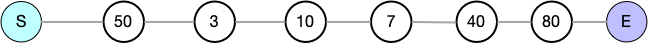
\includegraphics[scale=0.55]{fig/LIS_1.png}
\end{figure}\label{fig:LIS1}

图中玩家选择3,7,40,80将得到最多的得分4。

\bparts
\ppart 如果各个棋子的分值是10, 22, 9, 33, 21, 50, 41, 60, 80,那么玩家获胜的得分是多少?

这个问题实际上是求解最长递增子序列(LIS - Longest Increasing Subsequence)的问题。在跳棋游戏中,我们需要找到一个严格递增的序列,使得序列长度最大。注意,游戏的得分是跳跃次数,即序列的长度。

对于棋子分值10, 22, 9, 33, 21, 50, 41, 60, 80,我们需要找到其中的最长递增子序列。

使用动态规划算法分析:
\begin{enumerate}
    \item 定义dp[i]表示以第i个元素结尾的最长递增子序列的长度。
    \item 初始化dp[i] = 1(每个元素自身就是一个长度为1的递增子序列)。
    \item 对于每个位置i,考虑之前的所有位置j < i,如果nums[i] > nums[j],则可以将第i个元素接在以第j个元素结尾的序列之后,得到dp[i] = max(dp[i], dp[j] + 1)。
\end{enumerate}

计算过程:
\begin{align}
dp[0] &= 1 \quad \text{(10)} \\
dp[1] &= 2 \quad \text{(10, 22)} \\
dp[2] &= 1 \quad \text{(9)} \\
dp[3] &= 3 \quad \text{(10, 22, 33)} \\
dp[4] &= 2 \quad \text{(10, 21)} \\
dp[5] &= 4 \quad \text{(10, 22, 33, 50)} \\
dp[6] &= 4 \quad \text{(10, 22, 33, 41)} \\
dp[7] &= 5 \quad \text{(10, 22, 33, 50, 60)} \\
dp[8] &= 6 \quad \text{(10, 22, 33, 50, 60, 80)}
\end{align}

最长递增子序列是[10, 22, 33, 50, 60, 80],长度为6。因此,玩家获胜的得分是6。

\ppart 描述利用穷举法求解该问题的步骤,并给出其时间复杂度。

穷举法的基本思想是生成所有可能的递增子序列,并找出其中最长的一个。

算法步骤如下:
\begin{enumerate}
    \item 从起点开始,考虑两种选择:跳过当前棋子,或者选择当前棋子并继续跳跃。
    \item 如果选择当前棋子,下一步只能跳到值比当前值大的棋子上。
    \item 递归地探索所有可能的跳跃路径,并记录最长的路径长度。
\end{enumerate}

伪代码如下:
\begin{verbatim}
lis_brute_force(nums, curr_idx=0, prev_val=negative_infinity, curr_sequence=[]):
    # 基本情况:到达数组末尾
    if curr_idx == length(nums):
        return curr_sequence
    
    # 选择1:跳过当前数字
    skip_result = lis_brute_force(nums, curr_idx + 1, prev_val, curr_sequence)
    
    # 选择2:如果当前数字大于前一个选择的数字,则选择当前数字
    take_result = []
    if nums[curr_idx] > prev_val:
        new_sequence = curr_sequence + [nums[curr_idx]]
        take_result = lis_brute_force(nums, curr_idx + 1, nums[curr_idx], new_sequence)
    
    # 返回长度更大的序列
    if length(take_result) > length(skip_result):
        return take_result
    else:
        return skip_result
\end{verbatim}

时间复杂度分析:最坏情况下,对于每个位置,我们都需要考虑选择或不选择两种情况,因此时间复杂度为$O(2^n)$,其中$n$是棋子的数量。

\ppart 详细描述用动态规划求解该问题的步骤。

动态规划法的思想是利用问题的最优子结构性质,通过解决子问题来解决原问题。对于最长递增子序列问题,我们定义状态$dp[i]$表示以第$i$个元素结尾的最长递增子序列的长度。

算法步骤如下:
\begin{enumerate}
    \item 初始化dp数组,dp[i] = 1,表示每个元素自身就是一个长度为1的递增子序列。
    \item 对于每个位置i(从1到n-1),遍历所有之前的位置j(从0到i-1):
    \begin{itemize}
        \item 如果nums[i] > nums[j],则可以将第i个元素接在以第j个元素结尾的序列之后,得到dp[i] = max(dp[i], dp[j] + 1)。
    \end{itemize}
    \item 最终,最长递增子序列的长度是dp数组中的最大值。
\end{enumerate}

为了构建出实际的最长递增子序列,我们还需要记录每个位置的前一个元素的索引:
\begin{enumerate}
    \item 初始化prev数组,prev[i] = -1,表示没有前一个元素。
    \item 在更新dp[i]时,如果通过nums[j]得到更长的序列,则更新prev[i] = j。
    \item 通过回溯prev数组,我们可以构建出最长递增子序列。
\end{enumerate}

状态转移方程:
\begin{align}
dp[i] = \max_{j < i, nums[j] < nums[i]} \{dp[j] + 1\}
\end{align}

时间复杂度分析:有两层嵌套循环,因此时间复杂度为$O(n^2)$,其中$n$是棋子的数量。空间复杂度为$O(n)$。

\ppart 给出动态规划求解该问题的代码实现。

以下是使用Python实现的最长递增子序列的动态规划算法:

\begin{verbatim}
def lis_dp(nums):
    """
    动态规划法求解最长递增子序列
    时间复杂度:O(n^2),其中n是数组长度
    空间复杂度:O(n)
    """
    if not nums:
        return []
    
    n = len(nums)
    # dp[i]表示以第i个元素结尾的最长递增子序列的长度
    dp = [1] * n
    # prev[i]记录以第i个元素结尾的最长递增子序列的前一个元素的索引
    prev = [-1] * n
    
    # 填充dp数组
    for i in range(1, n):
        for j in range(i):
            if nums[i] > nums[j] and dp[i] < dp[j] + 1:
                dp[i] = dp[j] + 1
                prev[i] = j
    
    # 找到最长递增子序列的结束位置
    max_length = max(dp)
    end_index = dp.index(max_length)
    
    # 重建最长递增子序列
    lis = []
    while end_index != -1:
        lis.append(nums[end_index])
        end_index = prev[end_index]
    
    # 逆序返回,得到正确的顺序
    return list(reversed(lis))
\end{verbatim}

使用示例:

\begin{verbatim}
test_case = [10, 22, 9, 33, 21, 50, 41, 60, 80]
lis = lis_dp(test_case)
print(f"最长递增子序列: {lis}")
print(f"得分: {len(lis)}")
\end{verbatim}

对于上述例子,输出结果为:

\begin{verbatim}
最长递增子序列: [10, 22, 33, 50, 60, 80]
得分: 6
\end{verbatim}

这表示玩家应该按照10 → 22 → 33 → 50 → 60 → 80的顺序跳跃,得分为6。

此外,值得一提的是,最长递增子序列问题还有一个时间复杂度为$O(n \log n)$的优化算法,基于二分查找,在实际应用中更为高效:

\begin{verbatim}
def lis_dp_optimized(nums):
    """
    优化的动态规划法求解最长递增子序列
    时间复杂度:O(n log n),其中n是数组长度
    空间复杂度:O(n)
    """
    if not nums:
        return []
    
    n = len(nums)
    # tails[i]存储长度为i+1的递增子序列的最小结尾值
    tails = []
    # 记录每个元素所在的递增子序列长度
    length = [0] * n
    
    for i in range(n):
        # 二分查找:查找第一个大于等于nums[i]的位置
        left, right = 0, len(tails)
        while left < right:
            mid = (left + right) // 2
            if tails[mid] < nums[i]:
                left = mid + 1
            else:
                right = mid
                
        # 如果找不到,则添加到tails末尾
        if left == len(tails):
            tails.append(nums[i])
        else:
            tails[left] = nums[i]
            
        length[i] = left + 1
    
    # 重建最长递增子序列
    lis_length = len(tails)
    lis = [0] * lis_length
    curr_len = lis_length
    
    for i in range(n - 1, -1, -1):
        if length[i] == curr_len:
            lis[curr_len - 1] = nums[i]
            curr_len -= 1
            if curr_len == 0:
                break
    
    return lis
\end{verbatim}

\eparts

\end{problems}
\end{document}

